\paragraph{QuizziPedia::Back-End::App::Routers::QuizRouter}
\label{QuizziPedia::Back-End::App::Routers::QuizRouter}
\begin{figure}[ht]
	\centering
	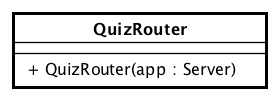
\includegraphics[scale=0.45]{UML/Classi/Back-End/QuizziPedia_Back-End_App_Routers_quizRouter.png}
	\caption{QuizziPedia::Back-End::App::Routers::QuizRouter}
\end{figure}
\FloatBarrier
	\begin{itemize}
		\item \textbf{Descrizione} \\
		Classe che gestisce le richieste relative alle operazioni riguardanti un questionario. Componente \textit{ConcreteHandler\ped{G}} del \textit{design pattern\ped{G}} \textit{Chain of responsibility\ped{G}};
		\item \textbf{Utilizzo} \\
		Viene utilizzata per chiamare il \textit{controller\ped{G}} che si occupa di gestire le \textit{API\ped{G}} relative ad un questionario;
		\item \textbf{Relazioni con altre classi} 
		\begin{itemize}
		\item \textbf{IN \texttt{Server}} \\
			Classe che avvia il \textit{server\ped{G}}. Nello specifico apre una connessione al database tramite \textit{Mongoose\ped{G}}, invoca il \textit{middleware\ped{G}} \textit{Express\ped{G}} passando un riferimento al database \textit{MongoDB\ped{G}} come parametro in modo che possa configurarsi con esso, invoca il \textit{middleware\ped{G}} \textit{Passport\ped{G}} ed infine si mette in ascolto su una determinata porta. È il componente client del \textit{design pattern\ped{G}} \textit{Chain of responsibility\ped{G}}. Utilizza i moduli \textit{Mongoose\ped{G}}, \textit{Express\ped{G}}, \textit{Passport\ped{G}};
		\item \textbf{OUT \texttt{ErrorHandler}} \\
			Classe \textit{middleware\ped{G}} per la gestione degli errori. Ritorna al client un oggetto di tipo \texttt{Response} con stato \textit{HTTP\ped{G}} 500 e descrizione dell'errore in formato \textit{JSON\ped{G}}. È un componente \textit{ConcreteHandler\ped{G}} del \textit{design pattern\ped{G}} \textit{Chain of responsibility\ped{G}};
		\item \textbf{OUT \texttt{NotFoundHandler}} \\
			Classe che si occupa della gestione dell'errore di pagina non trovata. Componente \textit{ConcreteHandler\ped{G}} del \textit{design pattern\ped{G}} \textit{Chain of responsibility\ped{G}};
		\item \textbf{OUT \texttt{QuizController}} \\
			Classe che raggruppa i vari \textit{controllers\ped{G}} responsabili delle operazioni riguardanti un questionario attraverso \texttt{require}.
		\end{itemize}
		\item \textbf{Metodi} 
		\begin{itemize}
		\item \texttt{+ QuizRouter(app: Server)} \\
		Contiene diverse \textit{route\ped{G}} che vengono configurate all'avvio del \textit{server\ped{G}}. Quest'ultime ricevono le richieste del client e passano il controllo al \textit{ConcreteHandler\ped{G}} successivo. \\
		\textbf{Parametri}:
		\begin{itemize}
		\item \texttt{app : Server} \\
		Rappresenta l'istanza del \textit{server\ped{G}} su cui configurare i \textit{route\ped{G}} che mappano i \textit{controllers\ped{G}} specifici.
		\end{itemize}
		\end{itemize}
	\end{itemize}